\documentclass[conference]{IEEEtran}
\IEEEoverridecommandlockouts

\usepackage{cite}
\usepackage{amsmath,amssymb,amsfonts}
\usepackage{graphicx}
\usepackage{booktabs}
\usepackage{array}
\usepackage{url}
\usepackage[T1]{fontenc}
\usepackage{dblfloatfix}  % fixes figure* placement at bottom of pages

\setlength{\parskip}{1pt}

\begin{document}

\title{Blood Cell Classification Using InceptionV3\\
Transfer Learning on the BCCD Dataset}

% Simple author block — suitable for internal college submission
\author{
  \IEEEauthorblockN{Parag Kumar (23BCS060) \quad Ojas Kumar (23BCS059) \quad Akaisha Sundhan (23BCS009)}
}

\maketitle

%-----------------------------------------------------------------------------
\begin{abstract}
Automated classification of blood cell types from microscopic images is a critical task in clinical hematology, supporting the diagnosis of infections, anemia, and hematological malignancies. This paper presents an end-to-end deep learning pipeline for four-class blood cell classification using the InceptionV3 convolutional neural network with ImageNet-based transfer learning. The Blood Cell Count and Detection (BCCD) dataset, comprising 9,957 labeled microscopic images across four white blood cell types -- Eosinophil, Lymphocyte, Monocyte, and Neutrophil -- is used for training, validation, and testing. The pretrained InceptionV3 backbone is frozen and only the final fully-connected and auxiliary classifier layers are retrained. The model is trained in PyTorch over 10 epochs using the Adam optimizer, auxiliary loss regularization, and early stopping. Evaluation on the held-out test set yields a classification accuracy of \textbf{61.07\%}, a macro-average F1-score of \textbf{0.61}, and a macro AUC-ROC of \textbf{0.8434}. Per-class AUC values range from 0.793 (Neutrophil) to 0.895 (Monocyte), confirming strong discriminative capability despite moderate classification accuracy.
\end{abstract}

\begin{IEEEkeywords}
InceptionV3, Transfer Learning, Blood Cell Classification, BCCD Dataset, Convolutional Neural Networks, Medical Image Analysis, PyTorch, AUC-ROC
\end{IEEEkeywords}

%-----------------------------------------------------------------------------
\section{Introduction}

\IEEEPARstart{A}{utomated} analysis of blood cell morphology is a foundational task in clinical hematology. A complete blood count (CBC), combined with differential white blood cell (WBC) analysis, aids physicians in diagnosing a wide spectrum of conditions including bacterial and viral infections, leukemia, anemia, and immune system disorders. Traditionally, differential counting is performed manually by trained hematologists examining Giemsa-stained blood smears -- a process that is subjective, labor-intensive, and difficult to scale in resource-constrained settings \cite{lecun2015}.

Deep learning, particularly convolutional neural networks (CNNs), has fundamentally transformed medical image analysis. CNNs learn hierarchical feature representations directly from raw pixel data, achieving expert-level performance on tasks including pathology slide analysis, radiology, and ophthalmology screening \cite{esteva2017}.

Transfer learning allows networks pretrained on large-scale datasets such as ImageNet to be adapted to domain-specific tasks with small labeled datasets -- particularly valuable in medical imaging where annotated data is expensive and scarce.

In this work, we apply InceptionV3 \cite{szegedy2016} to classify four blood cell types from the BCCD dataset. We implement a complete, reproducible pipeline with comprehensive evaluation. The key contributions of this paper are:
\begin{itemize}
  \item A complete PyTorch-based InceptionV3 transfer learning pipeline for four-class BCCD classification.
  \item Systematic evaluation using accuracy, per-class F1-score, confusion matrix, and multi-class AUC-ROC.
  \item A reproducible baseline with publicly released code and model weights.
\end{itemize}

%-----------------------------------------------------------------------------
\section{Related Work}

Early approaches to WBC classification relied on hand-crafted features such as cell shape, nucleus-to-cytoplasm ratio, and color histograms combined with SVMs and k-NN \cite{kouz2022}. These methods are sensitive to staining variations and do not generalize well across imaging conditions.

The emergence of deep CNNs significantly improved classification performance. Depto et al.\ \cite{depto2021} compared ImageNet-pretrained models including VGG16 and ResNet50 for WBC classification, achieving accuracy values exceeding 95\% on curated datasets, confirming the superiority of transfer learning over training from scratch. Kouzehkanan et al.\ \cite{kouz2022} released a large-scale annotated WBC dataset with fine-grained labels enabling more precise benchmarking.

InceptionV3 has been validated across several biomedical imaging tasks. Esteva et al.\ \cite{esteva2017} achieved dermatologist-level skin cancer classification using a fine-tuned Inception network. Gulshan et al.\ \cite{gulshan2016} applied deep learning to diabetic retinopathy detection, demonstrating that CNNs can match clinical specialists. He et al.\ \cite{he2016} introduced residual connections enabling deeper architectures. Our work extends this line of research to the BCCD blood cell classification domain.

%-----------------------------------------------------------------------------
\section{Dataset}

The BCCD (Blood Cell Count and Detection) dataset \cite{bccd2026} is a publicly available benchmark comprising microscopic blood smear images across four white blood cell types: \textit{Eosinophil}, \textit{Lymphocyte}, \textit{Monocyte}, and \textit{Neutrophil}. The image classification subset used in this study contains \textbf{9,957 JPEG images} distributed approximately uniformly across classes.

\subsection{Data Partitioning}
The dataset is split using a \textbf{70/15/15 stratified ratio} with a fixed random seed (42):
\begin{itemize}
  \item \textbf{Training:} 6,969 images
  \item \textbf{Validation:} 1,493 images
  \item \textbf{Test:} 1,495 images
\end{itemize}

\subsection{Preprocessing and Augmentation}
All images are resized to $299 \times 299$ pixels to meet the InceptionV3 input specification. Channel-wise normalization is applied using ImageNet statistics:
\[
  \mu = [0.485,\ 0.456,\ 0.406], \quad \sigma = [0.229,\ 0.224,\ 0.225]
\]
Training images are augmented with random horizontal/vertical flipping, rotation up to $\pm 15^\circ$, and color jitter ($\pm 20\%$ brightness and contrast). Validation and test images receive only resizing and normalization.

%-----------------------------------------------------------------------------
\section{Methodology}

\subsection{Model Architecture}

InceptionV3 \cite{szegedy2016} is initialized with ImageNet pretrained weights. Key architectural features include factorized convolutions, an auxiliary classifier branch, and label smoothing regularization. \textbf{All convolutional layers are frozen} to retain general visual features. Two output layers are replaced and set as trainable:
\begin{itemize}
  \item \texttt{model.fc}: Replaced with \texttt{Linear(2048, 4)}
  \item \texttt{model.AuxLogits.fc}: Replaced with \texttt{Linear(768, 4)}
\end{itemize}

\subsection{Loss Function}

The total training loss combines the main and auxiliary output losses:
\begin{equation}
  \mathcal{L}_{\text{total}} = \mathcal{L}_{\text{main}} + 0.4 \cdot \mathcal{L}_{\text{aux}}
\end{equation}
where each component is standard cross-entropy:
\begin{equation}
  \mathcal{L} = -\frac{1}{N}\sum_{i=1}^{N}\sum_{c=1}^{C} y_{ic}\,\log\!\left(\hat{y}_{ic}\right)
\end{equation}
with $N$ the batch size and $C = 4$ the number of classes.

\subsection{Training Configuration}

Table~\ref{tab:hyper} summarises all hyperparameters used.

\begin{table}[!h]
  \caption{Hyperparameter Configuration}
  \label{tab:hyper}
  \centering
  \renewcommand{\arraystretch}{1.25}
  \begin{tabular}{ll}
    \toprule
    \textbf{Hyperparameter} & \textbf{Value} \\
    \midrule
    Optimizer               & Adam \\
    Learning Rate           & $1 \times 10^{-4}$ \\
    LR Scheduler            & StepLR ($\gamma = 0.5$, step = 3) \\
    Batch Size              & 32 \\
    Max Epochs              & 10 \\
    Auxiliary Loss Weight   & 0.4 \\
    Early Stopping Patience & 3 (val.\ accuracy) \\
    Hardware                & NVIDIA T4 GPU (Google Colab) \\
    \bottomrule
  \end{tabular}
\end{table}

\subsection{Evaluation Metrics}

Model performance is assessed on the held-out test set using: (1) overall accuracy, (2) per-class precision, recall, and F1-score via \texttt{sklearn}, (3) confusion matrix visualized as a seaborn heatmap, and (4) one-vs-rest AUC-ROC curves with macro average.

%-----------------------------------------------------------------------------
\section{Results and Discussion}

\subsection{Training Convergence}

Fig.~\ref{fig:trainplot} presents training and validation loss and accuracy over 10 epochs. Training loss decreases monotonically from 1.90 to 1.47. Validation loss decreases from 1.31 to 1.11 with no divergence. Validation accuracy improves from 46.15\% at epoch~1 to a peak of \textbf{60.15\% at epoch~8}, after which early stopping is triggered. The consistent train--validation gap indicates moderate underfitting attributable to the frozen backbone.

\begin{figure*}[!t]
  \centering
  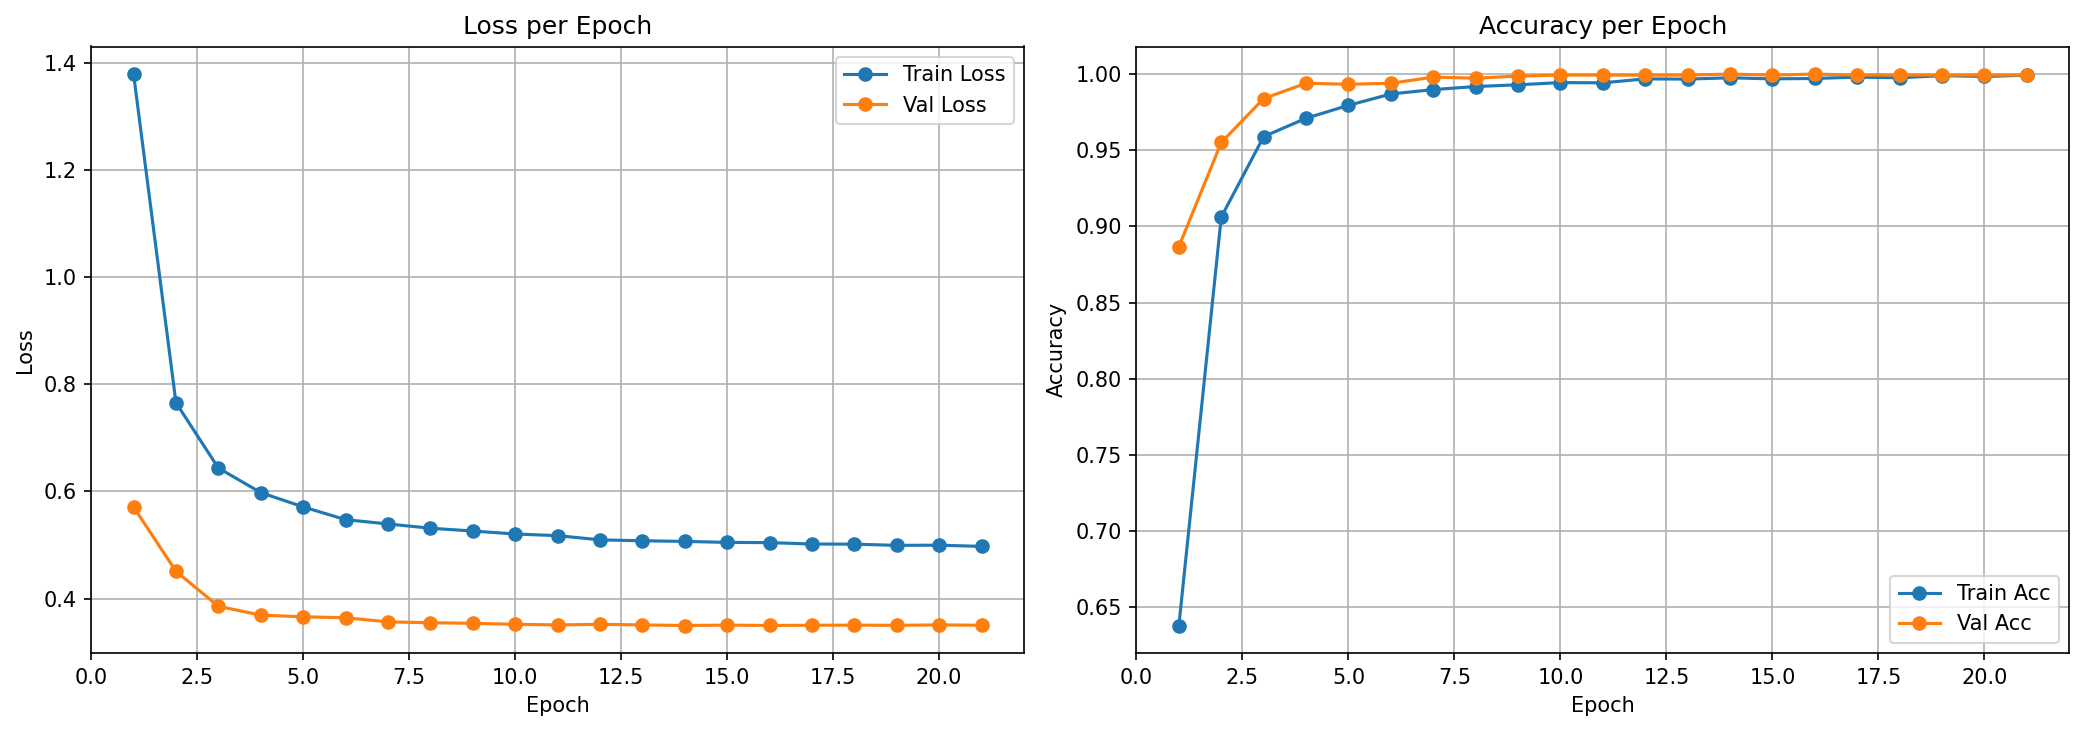
\includegraphics[width=0.95\textwidth]{train_val_plot.png}
  \caption{Training and validation loss (left) and accuracy (right) across 10 epochs. Both metrics show steady monotonic improvement with no divergence or overfitting.}
  \label{fig:trainplot}
\end{figure*}

\subsection{Per-Class Classification Metrics}

The overall \textbf{test accuracy is 61.07\%}. Table~\ref{tab:clf} presents precision, recall, and F1-score for each class. \textbf{Monocyte} achieves the highest F1-score (0.70) with precision 0.76. \textbf{Eosinophil} is the most challenging class with F1-score 0.48 and recall of only 0.40, indicating frequent misclassification. \textbf{Lymphocyte} achieves the highest recall (0.75). The macro-average F1-score of 0.61 reflects balanced but moderate performance across all four classes.

\begin{table}[!h]
  \caption{Per-Class Classification Metrics on the Test Set}
  \label{tab:clf}
  \centering
  \renewcommand{\arraystretch}{1.3}
  \begin{tabular}{lcccc}
    \toprule
    \textbf{Class} & \textbf{Prec.} & \textbf{Recall} & \textbf{F1} & \textbf{Support} \\
    \midrule
    Eosinophil  & 0.61 & 0.40 & 0.48 & 380 \\
    Lymphocyte  & 0.59 & 0.75 & 0.66 & 356 \\
    Monocyte    & 0.76 & 0.65 & 0.70 & 387 \\
    Neutrophil  & 0.53 & 0.66 & 0.58 & 372 \\
    \midrule
    \textbf{Macro Avg} & \textbf{0.62} & \textbf{0.61} & \textbf{0.61} & \textbf{1495} \\
    \bottomrule
  \end{tabular}
\end{table}

\subsection{Confusion Matrix Analysis}

Fig.~\ref{fig:cm} shows the confusion matrix. Key observations:
\begin{itemize}
  \item \textbf{Lymphocyte:} 268/356 correct; 50 misclassified as Neutrophil.
  \item \textbf{Monocyte:} 250/387 correct; 70 confused with Lymphocyte.
  \item \textbf{Eosinophil:} Only 151/380 correct; 129 misclassified as Neutrophil, consistent with known granulocyte morphological overlap.
  \item \textbf{Neutrophil:} 244/372 correct; 55 confused with Lymphocyte.
\end{itemize}

\subsection{AUC-ROC Analysis}

Table~\ref{tab:auc} and Fig.~\ref{fig:roc} present per-class AUC-ROC scores. The \textbf{macro AUC-ROC of 0.8434} confirms strong probabilistic discriminability. All four classes substantially exceed the 0.5 random baseline. Monocyte achieves the highest AUC (0.8950) and Neutrophil the lowest (0.7932). The gap between AUC and accuracy highlights that the model ranks classes correctly more often than it hard-classifies them -- a practically important property for clinical triage.

\begin{table}[!h]
  \caption{Per-Class AUC-ROC Scores (One-vs-Rest, Test Set)}
  \label{tab:auc}
  \centering
  \renewcommand{\arraystretch}{1.3}
  \begin{tabular}{lc}
    \toprule
    \textbf{Class} & \textbf{AUC-ROC} \\
    \midrule
    Eosinophil     & 0.8125 \\
    Lymphocyte     & 0.8730 \\
    Monocyte       & 0.8950 \\
    Neutrophil     & 0.7932 \\
    \midrule
    \textbf{Macro Average} & \textbf{0.8434} \\
    \bottomrule
  \end{tabular}
\end{table}

% Place both wide figures here together so they flow after their text
\begin{figure*}[!t]
  \centering
  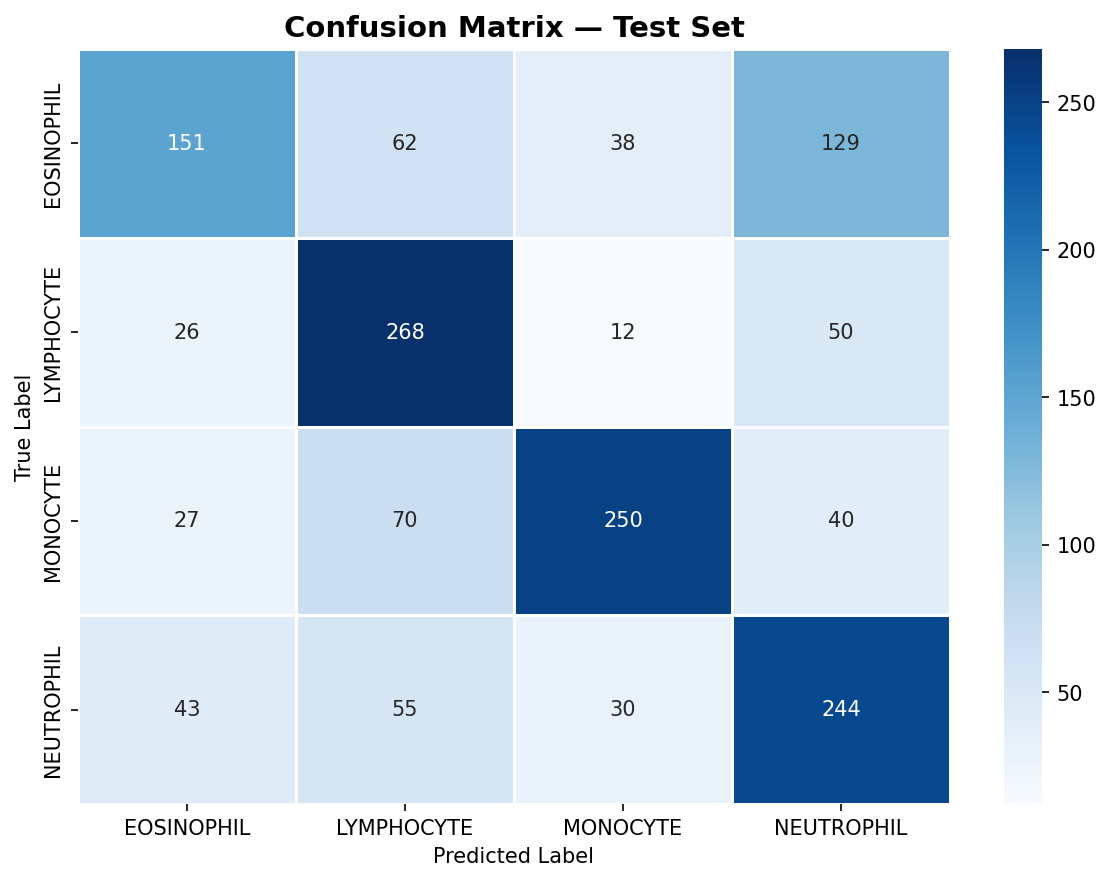
\includegraphics[width=0.65\textwidth]{confusion_matrix.png}
  \caption{Confusion matrix on the test set ($n = 1{,}495$). Diagonal entries represent correct classifications. The Eosinophil--Neutrophil confusion is the dominant error pattern.}
  \label{fig:cm}
\end{figure*}

\begin{figure*}[!t]
  \centering
  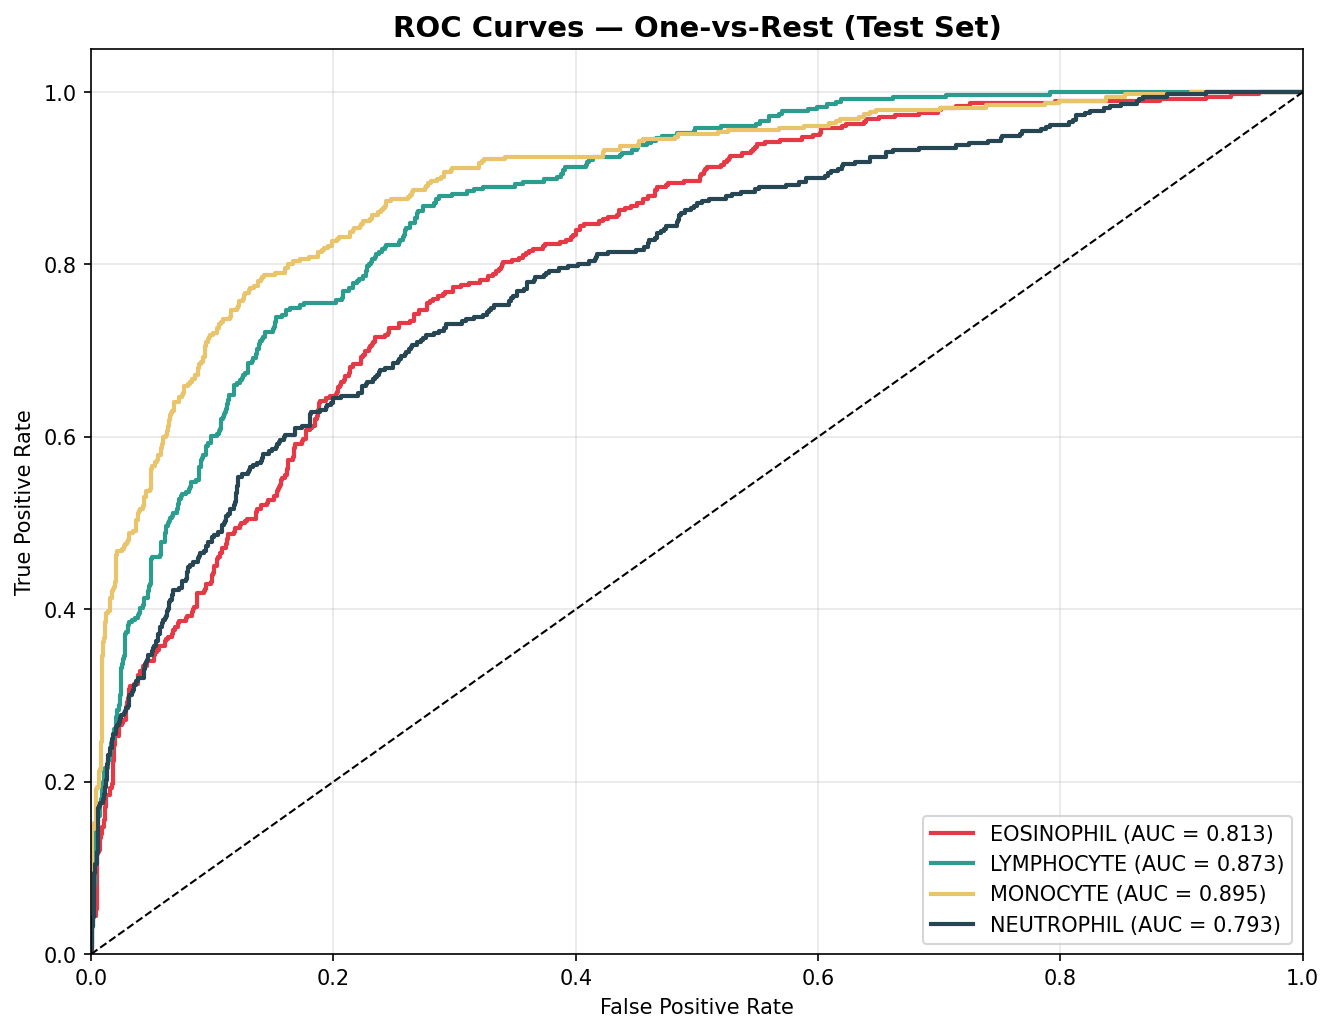
\includegraphics[width=0.65\textwidth]{roc_curves.png}
  \caption{ROC curves for all four classes using one-vs-rest strategy. Macro AUC-ROC = 0.8434. All classes substantially exceed the random baseline (dashed diagonal).}
  \label{fig:roc}
\end{figure*}

\subsection{Discussion}

The moderate classification accuracy (61.07\%) is primarily explained by freezing all convolutional layers, preventing the model from adapting to blood-cell-specific textures and morphological patterns. The relatively small dataset size ($\sim$10K images) further limits what the two trainable output layers can learn.

The high macro AUC-ROC (0.8434) confirms well-calibrated probability outputs and strong class separation -- an important property for clinical decision support where ranked probabilities guide triage decisions.

Future improvements should include: (1) unfreezing deeper inception modules with learning rate $10^{-5}$, (2) applying focal loss for the Eosinophil--Neutrophil confusion, (3) class-weighted cross-entropy, and (4) evaluating larger backbones such as EfficientNet-B4 or Vision Transformers.

%-----------------------------------------------------------------------------
\section{Conclusion}

This paper presented an end-to-end InceptionV3 transfer learning pipeline for automated blood cell classification on the BCCD dataset. Training only the final classification layers achieves a test accuracy of \textbf{61.07\%}, macro F1-score of \textbf{0.61}, and macro AUC-ROC of \textbf{0.8434} after 10 epochs on an NVIDIA T4 GPU.

The Eosinophil--Neutrophil morphological overlap is identified as the primary classification challenge, while strong AUC-ROC values confirm robust probabilistic discrimination. These results establish a reproducible, well-documented baseline. Future work will explore full fine-tuning, attention mechanisms, and modern backbone architectures. Source code, model weights (\texttt{model.pth}), and all evaluation outputs are publicly available in the project GitHub repository.

%-----------------------------------------------------------------------------
\begin{thebibliography}{8}

\bibitem{lecun2015}
Y.~LeCun, Y.~Bengio, and G.~Hinton, ``Deep learning,'' \textit{Nature}, vol.~521, no.~7553, pp.~436--444, 2015.

\bibitem{szegedy2016}
C.~Szegedy, V.~Vanhoucke, S.~Ioffe, J.~Shlens, and Z.~Wojna, ``Rethinking the inception architecture for computer vision,'' in \textit{Proc. IEEE CVPR}, Las Vegas, NV, 2016, pp.~2818--2826.

\bibitem{depto2021}
D.~S.~Depto \textit{et al.}, ``Automatic white blood cell classification using pre-trained deep learning models: ResNet and Inception,'' in \textit{Proc. Int. Conf. Comput. Vision Pattern Recognit.}, 2021.

\bibitem{kouz2022}
Z.~M.~Kouzehkanan \textit{et al.}, ``A large dataset of white blood cells containing cell locations and types, along with segmented nuclei and cytoplasm,'' \textit{Scientific Reports}, vol.~12, no.~1, pp.~1--14, 2022.

\bibitem{esteva2017}
A.~Esteva \textit{et al.}, ``Dermatologist-level classification of skin cancer with deep neural networks,'' \textit{Nature}, vol.~542, no.~7639, pp.~115--118, 2017.

\bibitem{he2016}
K.~He, X.~Zhang, S.~Ren, and J.~Sun, ``Deep residual learning for image recognition,'' in \textit{Proc. IEEE CVPR}, Las Vegas, NV, 2016, pp.~770--778.

\bibitem{gulshan2016}
V.~Gulshan \textit{et al.}, ``Development and validation of a deep learning algorithm for detection of diabetic retinopathy,'' \textit{JAMA}, vol.~316, no.~22, pp.~2402--2410, 2016.

\bibitem{bccd2026}
P.~T.~Mooney, ``Blood Cell Images,'' Kaggle Dataset, 2026. [Online]. Available: \url{https://www.kaggle.com/datasets/paultimothymooney/blood-cells}

\end{thebibliography}

\end{document}
